\documentclass[11pt,a4paper]{article}

\usepackage[T1]{fontenc}
\usepackage{amsmath}
\usepackage{booktabs}
\usepackage{cite}
\usepackage[margin=2.5cm]{geometry}
\usepackage{graphicx}
\usepackage{microtype}
\usepackage{mathptmx}
\usepackage{url}
\usepackage[hidelinks]{hyperref}

\setlength{\parindent}{0pt}
\setlength{\parskip}{0.55em}
\setlength{\floatsep}{1.1em}
\setlength{\textfloatsep}{1.2em}
\setlength{\intextsep}{1.1em}
\setlength{\emergencystretch}{2em}
\renewcommand{\arraystretch}{1.15}
\setcounter{tocdepth}{2}

\makeatletter
\setlength{\@fptop}{0pt}
\setlength{\@fpsep}{1.5em}
\setlength{\@fpbot}{0pt plus 1fil}
\makeatother

\newcommand{\reporttitle}{Leakage-Aware MLP Regression for Ames Housing:\\[0.35em]
A Controlled Comparison with Classical Baselines}

\begin{document}

\hypersetup{pageanchor=false}
\begin{titlepage}
\centering
\vspace*{1.0cm}
{\Large\bfseries Universidad Distrital Francisco Jos\'e de Caldas\par}
\vspace{0.55cm}
{\large Faculty of Engineering\par}
{\large Computer Engineering Program\par}

\vfill
{\Large\bfseries Workshop 2 -- Advanced Learning Models (Part A)\par}
\vspace{0.8cm}
{\LARGE\bfseries \reporttitle\par}

\vfill
{\large\bfseries Group 1 Authors\par}
\vspace{0.5cm}
{\large Miguel Alejandro Ch\'avez Porras -- 20212020033\par}
{\large Luisa Fernanda Guerrero Ordo\~nez -- 20212020099\par}
{\large Dilan Stive Arboleda Zambrano -- 20212020105\par}

\vfill
{\large Machine Learning -- Semester 2026-III\par}
{\large Bogot\'a, Colombia\par}
\vspace{0.5cm}
{\large 2026\par}
\end{titlepage}

\hypersetup{pageanchor=true}
\pagenumbering{roman}
\tableofcontents
\clearpage
\pagenumbering{arabic}

\begin{abstract}
Residential price prediction from heterogeneous tabular data requires nonlinear modeling while remaining robust to skewed targets, sparse categories, and rare high-value transactions. This work develops a leakage-aware multilayer perceptron (MLP) for the Ames Housing dataset, diagnoses an initial optimization failure, and evaluates controlled changes in architecture, dropout, weight decay, learning rate, and train-only standardization. The selected 261-128-64-1 network achieved a test mean absolute error (MAE) of \$14,666.23 on 440 held-out properties, improving the Workshop 1 Ridge, Random Forest, and Gradient Boosting baselines by 2.43\%, 12.18\%, and 1.42\%, respectively. Random Forest nevertheless retained the best root mean squared error and coefficient of determination, while Gradient Boosting retained the best logarithmic error. The results show that target conditioning and stable validation procedures can make an MLP competitive on a small tabular dataset, but do not establish universal neural-network superiority.
\end{abstract}

\noindent\textbf{Keywords:} Ames Housing, multilayer perceptron, regression, tabular data, reproducibility, model comparison.

\section{Introduction}
Automated residential valuation supports taxation, lending, investment, and market analysis, but accurate estimation is difficult because price depends on heterogeneous physical, temporal, quality, amenity, and location attributes. Ames Housing was introduced by De Cock as a modern alternative to the Boston Housing dataset and contains 2,930 sales recorded in Ames, Iowa, from 2006 to 2010, with 80 explanatory variables spanning nominal, ordinal, discrete, and continuous measurements \cite{decock2011}. Structural missingness, rare categories, nonlinear interactions, and a right-skewed price distribution make it a useful supervised-regression benchmark.

Workshop 1 established three classical baselines. Ridge Regression controls linear-model variance through coefficient shrinkage; Random Forest averages randomized trees \cite{breiman2001}; and Gradient Boosting constructs an additive predictor through stagewise functional optimization \cite{friedman2001}. All were implemented with scikit-learn \cite{pedregosa2011} and evaluated on a fixed split. They remain strong references because tabular benchmarks show that tree ensembles frequently match or outperform neural networks on small and medium datasets \cite{gorishniy2021,grinsztajn2022}.

An MLP is nevertheless an appropriate complementary model because successive affine transformations and nonlinear activations can approximate complex multivariate functions \cite{hornik1989}. Rectified linear units (ReLU) provide a simple non-saturating activation \cite{nair2010}, while Kaiming initialization stabilizes signal propagation through rectifier networks \cite{he2015}. With limited observations, flexibility must be controlled: dropout discourages hidden-unit co-adaptation \cite{srivastava2014}, Adam supplies adaptive first- and second-moment optimization \cite{kingma2015}, AdamW decouples weight decay from the adaptive update \cite{loshchilov2019}, and validation-based early stopping limits unnecessary fitting \cite{prechelt1998}. The implementation uses PyTorch \cite{paszke2019}.

This study asks whether a carefully conditioned MLP can improve the Workshop 1 baselines under the same observations and metric definitions. Its contributions are: (i) diagnosis of a failed initial run; (ii) a controlled architecture, regularization, learning-rate, and standardization comparison; (iii) ablations of input and target standardization; (iv) multi-seed stability analysis; and (v) one final evaluation of a checkpoint frozen using validation only. The goal is a reproducible, metric-aware comparison rather than a claim that deep learning is intrinsically superior.

\section{Methods and Materials}

\subsection{Dataset and Leakage-Aware Preprocessing}
The raw table contains 2,930 observations, 80 predictors, and the target \texttt{SalePrice}. Prices range from \$12,789 to \$755,000, with median \$160,000 and mean \$180,796. Twenty-seven columns contain missing values; many denote the physical absence of a pool, garage, basement, fireplace, alley, or fence rather than an unknown measurement.

The immutable \texttt{data/splits.json} assigns 2,050 records to training and 440 each to validation and test, approximately 70/15/15. The Workshop 1 preprocessor is fitted on training only. Two atypical training transactions with above-ground living area over 4,000 square feet and price below \$300,000 are removed, leaving 2,048 effective training examples; validation and test remain unfiltered. Structural absence is encoded as ``None'' or zero, lot frontage is imputed with neighborhood medians learned from training, other missing values use training modes or medians, ordered categories receive monotonic encodings, nominal variables are one-hot encoded with unknown categories ignored, and numerical variables are robustly scaled.

Feature engineering adds total usable area, weighted bathrooms, house and remodeling ages, porch area, amenity indicators, and a quality-condition interaction. The resulting matrix has 261 inputs. A diagnostic revealed that robust scaling alone left 741 training values with magnitude above 100 because several near-zero-interquartile-range variables retained large scales; \texttt{Misc Val} reached 15,500. Consequently, a second mean-standard-deviation transform was fitted to the processed training matrix and applied unchanged to validation and test.

The target is first mapped to $y_{\log}=\log(1+y)$ and then standardized with training statistics:
\begin{equation}
z_y=\frac{y_{\log}-\mu_{\mathrm{train}}}{\sigma_{\mathrm{train}}},
\end{equation}
where $\mu_{\mathrm{train}}=12.013993$ and $\sigma_{\mathrm{train}}=0.395353$. Inference returns predictions to dollars using
\begin{equation}
\hat y=\exp(\hat z_y\sigma_{\mathrm{train}}+\mu_{\mathrm{train}})-1.
\end{equation}
Every imputation, encoding, and scaling statistic is therefore learned without validation or test information.

\begin{figure}[htbp]
\centering
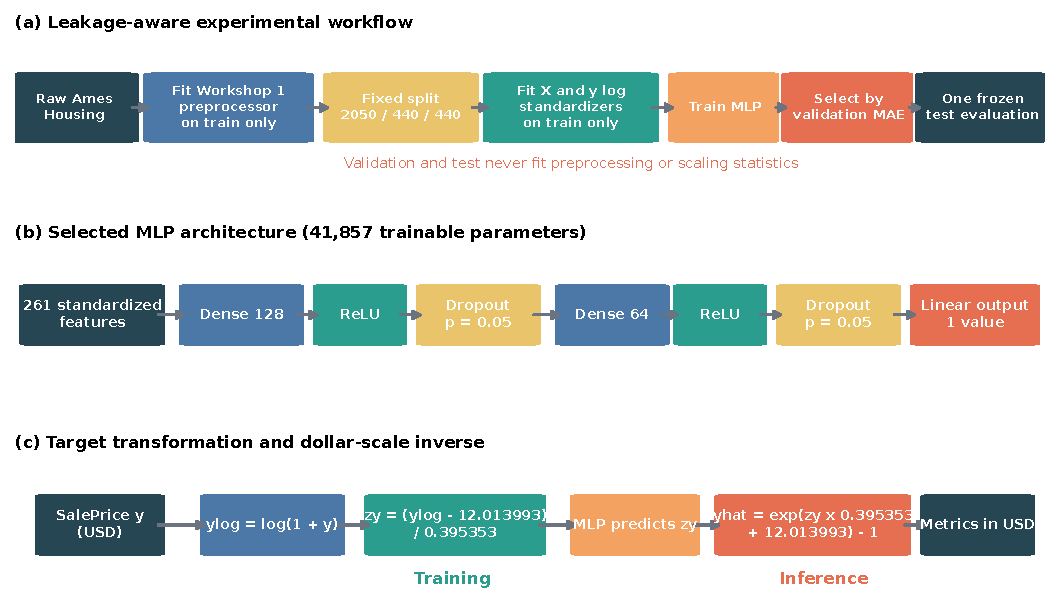
\includegraphics[width=0.98\textwidth]{figures/methodology_overview.pdf}
\caption{Leakage-aware methodology. (a) Data operations and selection order; (b) exact selected architecture, including dropout after both hidden ReLU layers; and (c) training-target transformation and inverse mapping used before dollar-scale metrics.}
\label{fig:methodology}
\end{figure}

\subsection{Network and Training Protocol}
Figure~\ref{fig:methodology} summarizes the complete workflow and selected architecture. The final MLP maps 261 inputs through hidden layers of 128 and 64 ReLU units. Dropout with probability 0.05 follows each hidden activation, and a final linear unit predicts the standardized log target. The model contains 41,857 trainable parameters. Hidden weights use Kaiming normal initialization, the output weights use Xavier uniform initialization, and all biases start at zero.

Training minimizes MSE on $z_y$. AdamW uses learning rate $10^{-3}$ and weight decay $10^{-5}$. Mini-batches contain 32 observations; gradient norm is clipped at 5. A ReduceLROnPlateau scheduler halves the learning rate after eight validation-loss plateaus, with minimum $10^{-5}$. Runs are allowed 250 epochs. Early stopping monitors validation MAE in dollars with patience 30, while the scheduler monitors validation MSE on the model scale. Seeds control Python, NumPy, PyTorch, and mini-batch order. The saved checkpoint contains model weights, architecture, feature order, split metadata, and both training-only standardizers.

\section{Experimental Setup}

\subsection{Initial Failure and Conditioning Correction}
The initial network used hidden widths 128-64-32, dropout 0.20, Adam, learning rate $10^{-3}$, and 43,905 parameters. It optimized MSE directly on $\log(1+\mathrm{SalePrice})$ without additional input or target standardization. Validation loss oscillated between 1.093 and 16.563, early stopping occurred after 36 epochs, and the best MAE was \$77,990.05 with negative $R^2$. This behavior is consistent with an output initialized near zero being asked to approximate an uncentered target near 12 while large feature magnitudes dominate early gradients.

Experiment 2 introduced train-only standardization of inputs and target, reduced the network to 64-32, lowered dropout to 0.05, changed Adam to AdamW, and added matched initialization, scheduling, and clipping. Table~\ref{tab:initial} shows the resulting 79.69\% MAE reduction. Because multiple changes were applied together, subsequent controlled experiments isolated their effects where possible.

\begin{table}[htbp]
\caption{Initial Diagnosis and Corrected Reference}
\label{tab:initial}
\centering
\small
\begin{tabular}{lrr}
\toprule
Validation result & Initial MLP & Experiment 2 \\
\midrule
Hidden units & 128-64-32 & 64-32 \\
Parameters & 43,905 & 18,881 \\
Best epoch & 16 & 75 \\
MAE (USD) & 77,990.05 & 15,837.95 \\
RMSE (USD) & 174,526.51 & 24,233.63 \\
$R^2$ & -2.9268 & 0.9243 \\
\bottomrule
\end{tabular}
\end{table}

\subsection{Controlled Comparison, Ablations, and Selection}
All seed-42 comparisons reuse the same 2,048 effective training rows and 440 validation rows. The experiment-2 reference uses 64-32 hidden units, dropout 0.05, weight decay $10^{-5}$, and learning rate $10^{-3}$. Four runs change one factor: dropout to 0, architecture to 128-64, weight decay to $10^{-4}$, or learning rate to $5\times10^{-4}$. Two ablations remove the additional input standardization or target standardization.

\begin{table}[htbp]
\caption{Controlled Validation Experiments with Seed 42}
\label{tab:validation}
\centering
\small
\setlength{\tabcolsep}{3.5pt}
\begin{tabular}{llllrrrr}
\toprule
ID & Hidden units & Changed factor & Standardization & Parameters & Epoch & MAE (USD) & $R^2$ \\
\midrule
Reference & 64-32 & None & Inputs and target & 18,881 & 75 & 15,837.95 & 0.9243 \\
E3 & 64-32 & Dropout 0.00 & Inputs and target & 18,881 & 66 & 19,330.28 & 0.8921 \\
E4 & 128-64 & Architecture & Inputs and target & 41,857 & 83 & \textbf{14,051.46} & \textbf{0.9452} \\
E5 & 64-32 & Weight decay $10^{-4}$ & Inputs and target & 18,881 & 81 & 15,534.41 & 0.9280 \\
E6 & 64-32 & Learning rate $5\times10^{-4}$ & Inputs and target & 18,881 & 61 & 16,341.55 & 0.9188 \\
A1 & 64-32 & No extra input scaling & Target only & 18,881 & 75 & 15,696.59 & 0.9108 \\
A2 & 64-32 & No target scaling & Inputs only & 18,881 & 152 & 34,600.95 & 0.5847 \\
\bottomrule
\end{tabular}
\end{table}

The reference and the two strongest non-ablation alternatives were repeated with seeds 7, 42, and 2026. Configuration selection used the lowest mean validation MAE across the three seeds. The 128-64 model achieved $14,238.79\pm183.95$, compared with $14,379.15\pm1,037.55$ for weight decay $10^{-4}$ and $14,695.31\pm1,021.94$ for the reference. Although stronger weight decay produced the best single run (\$13,526.67 at seed 7), its variability made it a less reliable choice. Among the three already-selected 128-64 runs, seed 42 had the lowest validation MAE (\$14,051.46) and was frozen before test evaluation.

\section{Results and Discussion}

\subsection{Optimization, Ablation, and Stability Results}
Figure~\ref{fig:experiments}(a) shows that target and input conditioning eliminated the extreme validation-MAE trajectory of the initial run. In the controlled study, removing target standardization was the most damaging ablation: MAE increased to \$34,600.95 and the best epoch moved to 152. The output layer otherwise begins near zero while the target remains near 12, producing unnecessarily large initial errors. Removing additional input standardization increased first-epoch MAE from \$31,590.70 to \$74,448.73 and worsened final RMSE and $R^2$, although its single-seed minimum MAE remained close to the reference. Thus, target standardization is directly supported by the ablation, while input standardization is supported mainly as an optimization and tail-error safeguard.

Removing dropout worsened MAE by \$3,492.33, consistent with overfitting. Increasing weight decay improved the seed-42 reference by \$303.53 but was unstable across seeds. Lowering the initial learning rate worsened MAE by \$503.60. Expanding the network to 128-64 produced the most consistent gain: under seed 42 it reduced MAE by \$1,786.48 (11.28\%) relative to experiment 2, and across seeds it had the lowest mean and standard deviation. The learning curves in Fig.~\ref{fig:loss} also show a persistent train-validation gap, so the selected checkpoint is determined by validation MAE rather than final training loss.

\begin{figure}[htbp]
\centering
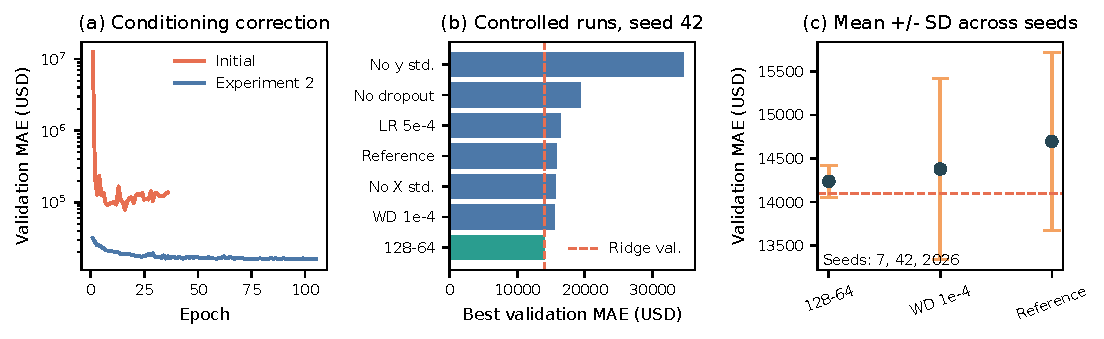
\includegraphics[width=0.98\textwidth]{figures/experimental_summary.pdf}
\caption{Optimization and model-selection evidence. (a) Validation MAE before and after conditioning; (b) controlled seed-42 comparison, including the Workshop 1 Ridge validation reference; and (c) mean $\pm$ standard deviation over seeds 7, 42, and 2026.}
\label{fig:experiments}
\end{figure}

\begin{figure}[htbp]
\centering
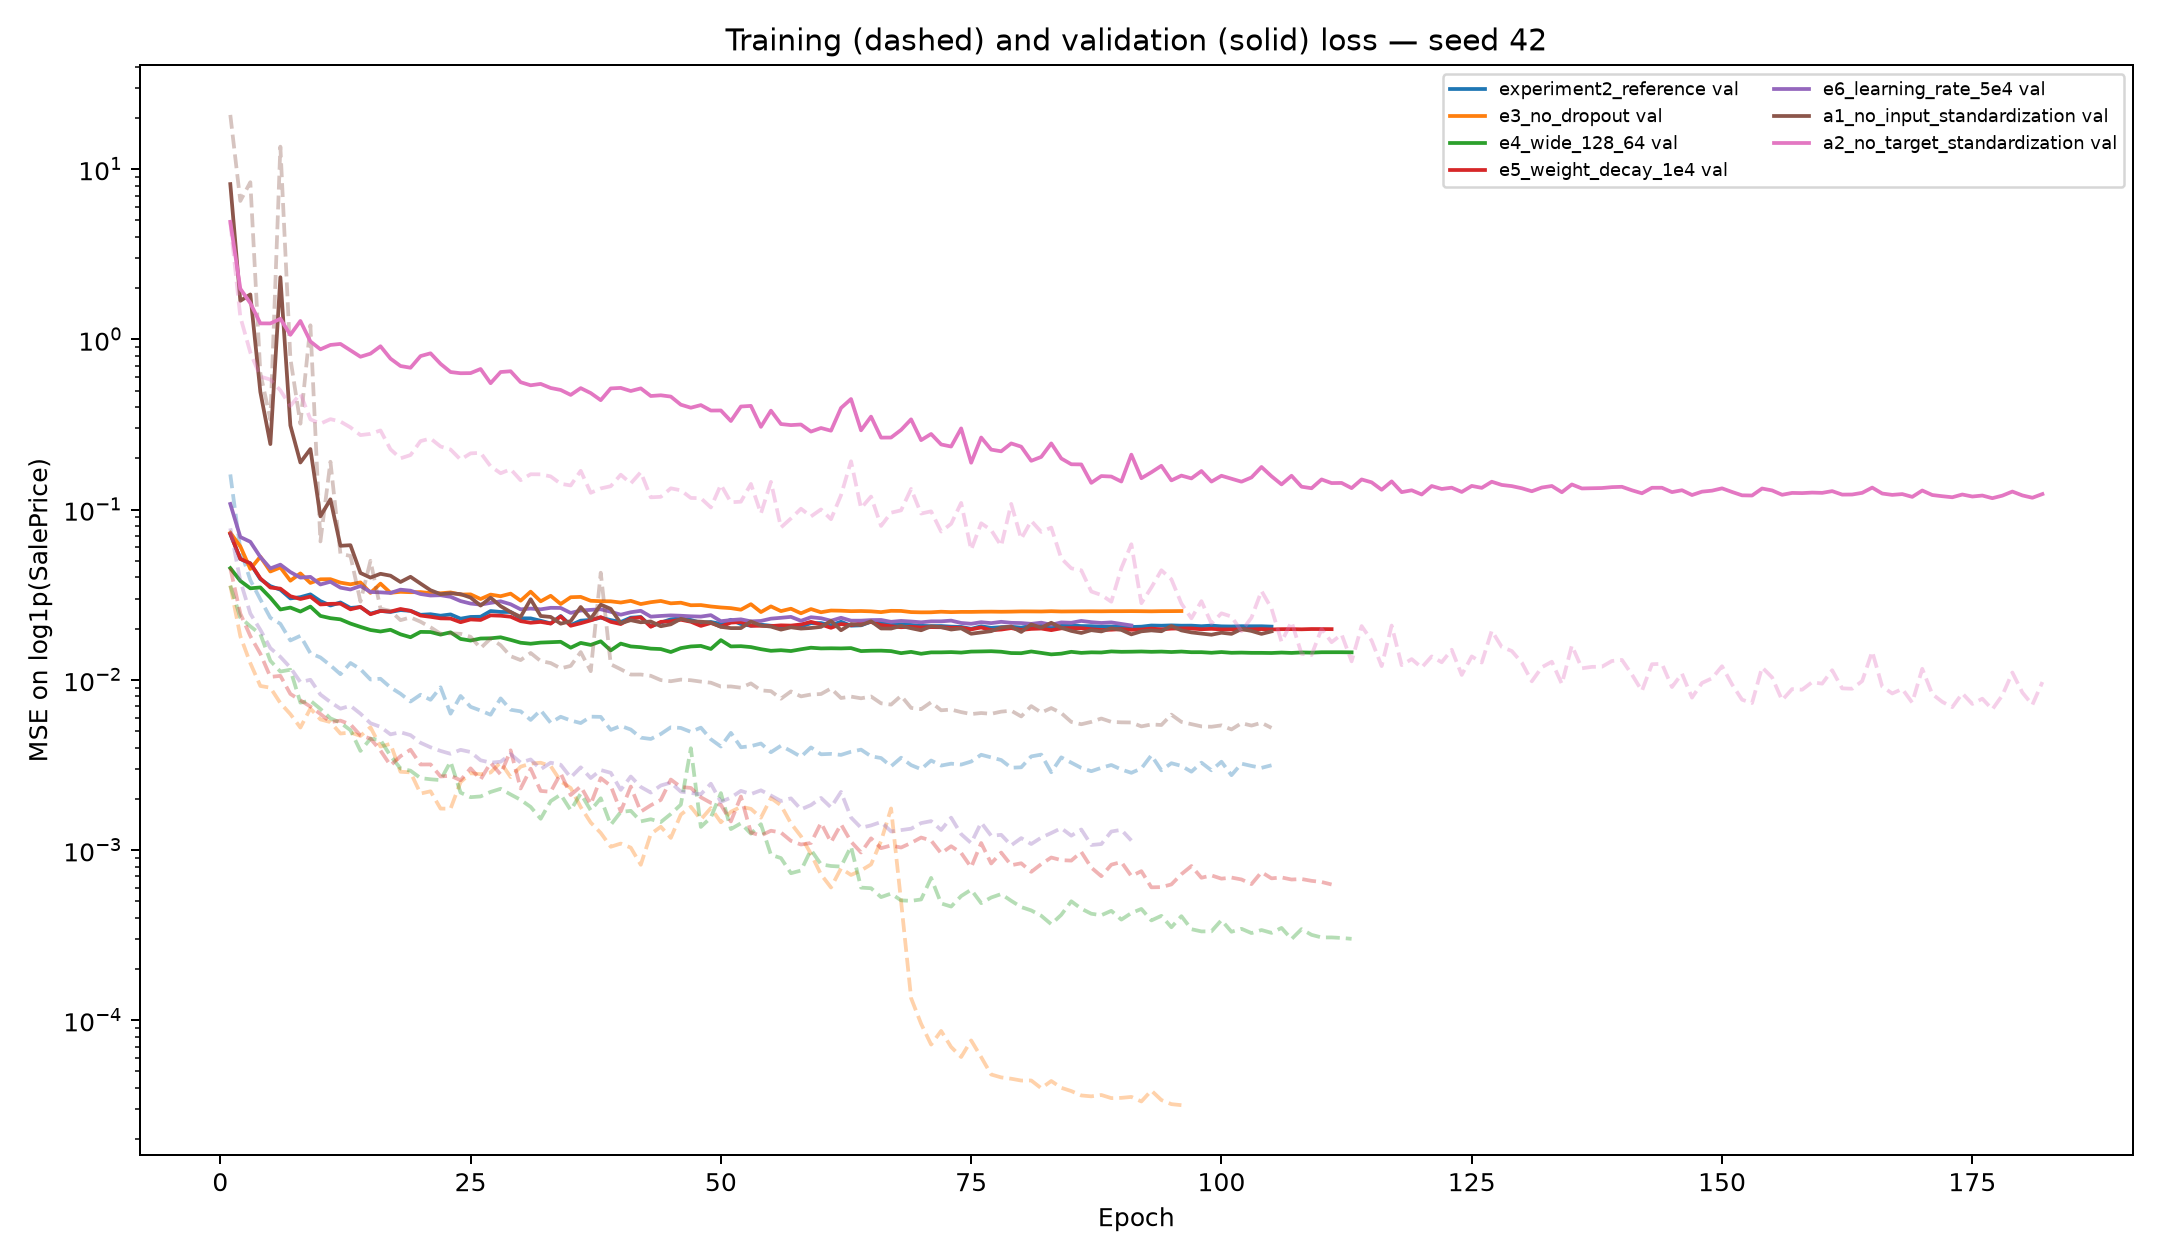
\includegraphics[width=0.96\textwidth]{../results/figures/part_a/loss_curves_seed42.png}
\caption{Training (dashed) and validation (solid) MSE for the controlled seed-42 experiments. The logarithmic vertical scale exposes the failed no-target-standardization ablation and the train-validation separation.}
\label{fig:loss}
\end{figure}

\begin{figure}[htbp]
\centering
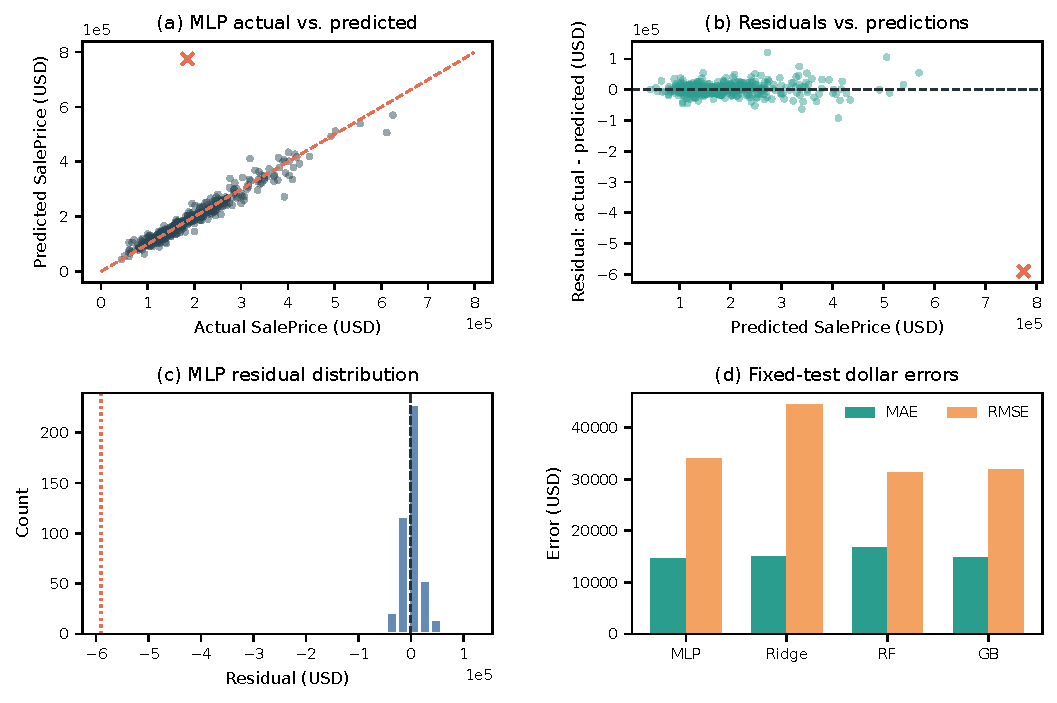
\includegraphics[width=0.94\textwidth]{figures/final_diagnostics.pdf}
\caption{Fixed-test diagnostics. (a) MLP actual versus predicted prices; (b) residuals versus predicted price; (c) residual distribution, with the extreme error marked; and (d) dollar-scale comparison with Workshop 1 baselines. Red crosses or dotted lines identify the largest absolute MLP residual.}
\label{fig:diagnostics}
\end{figure}

\subsection{Final Test Comparison}
The frozen seed-42 checkpoint was loaded without retraining and evaluated once on the 440 fixed test properties. Input normalization uses checkpoint statistics, and output inversion precedes all metrics. Table~\ref{tab:test} uses the immutable Workshop 1 test metrics and the new MLP metrics under the same definitions: MAE and RMSE in dollars, dollar-scale $R^2$, and RMSE on $\log(1+y)$.

\begin{table}[htbp]
\caption{Definitive Performance on the Fixed Test Partition ($N=440$)}
\label{tab:test}
\centering
\begin{tabular}{lrrrr}
\toprule
Model & MAE (USD) & RMSE (USD) & $R^2$ & RMSE$_{\log}$ \\
\midrule
Deep Learning MLP & \textbf{14,666.23} & 34,133.71 & 0.8483 & 0.1254 \\
Ridge Regression & 15,031.51 & 44,511.47 & 0.7421 & 0.1254 \\
Random Forest & 16,700.76 & \textbf{31,325.66} & \textbf{0.8723} & 0.1325 \\
Gradient Boosting & 14,876.80 & 31,939.29 & 0.8672 & \textbf{0.1208} \\
\bottomrule
\end{tabular}
\end{table}

The MLP achieved the smallest MAE, improving Ridge by \$365.28 (2.43\%), Random Forest by \$2,034.53 (12.18\%), and Gradient Boosting by \$210.57 (1.42\%). Its test MAE was 4.38\% above its validation MAE. The ranking changes with the metric: Random Forest obtained the best RMSE and $R^2$, while Gradient Boosting obtained the best logarithmic error. Therefore, the MLP improved typical absolute dollar deviation on this split but did not dominate squared-error or relative-error behavior.

\subsection{Predictions, Residuals, and Extreme Cases}
Figure~\ref{fig:diagnostics}(a) shows that most MLP predictions follow the identity line through the common price range. Residuals are concentrated near zero, with mean \$217, but their spread increases for expensive predictions. The largest error occurs at split index 2181 (PID 908154205): the actual price is \$184,750 and the MLP predicts \$775,256.31, producing residual $-\$590,506.31$. This unusual high-area, low-price property was retained in test by design and was not used to revise the model.

Because RMSE squares every residual before averaging, this single error contributes far more than a typical observation. It substantially increases MLP RMSE and lowers $R^2$, explaining how the network can lead in MAE while trailing both ensembles under tail-sensitive criteria. The diagnostic plots use reconstructed baseline predictions, whereas Table~\ref{tab:test} retains the historical Workshop 1 metrics.

\section{Reproducibility and Limitations}
The checkpoint was loaded into two independent model instances and produced identical prediction arrays. Seven final-evaluation tests verified validation-only selection, architecture metadata, training-only scaler statistics, the 440 ordered test indices, inverse target transformation, saved metric reproduction, and prediction-file identity. Three unit tests separately verified standardizer behavior, target round-trip accuracy, and model output shape. All ten tests passed, and the report notebook executes without retraining while rendering saved tables and figures.

The Workshop 1 baselines were reconstructed with frozen hyperparameters for diagnostic plots. In the current software environment their MAE values differed from the historical JSON by \$0.72 for Ridge, \$14.75 for Random Forest, and \$145.34 for Gradient Boosting. These small differences are consistent with numerical or library-version variation. To avoid presenting approximate reproduction as exact, the definitive table uses the immutable Workshop 1 metrics while the diagnostic plots use current predictions.

The evaluation has important limits. Only 2,048 effective training examples support 41,857 parameters. A single fixed split means seed repetitions measure initialization and mini-batch variability, not variation across data partitions. Only three configurations received multi-seed evaluation, so the search is controlled but not exhaustive. Test MAE across the three previously selected 128-64 checkpoints ranged from \$14,666.23 to \$16,746.04, with descriptive mean \$15,735.87 $\pm$ \$1,041.18; these values were not used to replace seed 42 or form an ensemble. Finally, the test set has now been observed and must not support further model selection.

\section{Conclusions}
A two-hidden-layer MLP can be competitive on Ames Housing when the processed inputs and log-transformed target are standardized using training statistics only. The initial failure demonstrates that a reasonable architecture and optimizer do not compensate for poor conditioning. Controlled experiments identified target standardization as the most important correction, light dropout as useful regularization, and 128-64 as the most stable evaluated architecture. Validation-only selection and checkpoint metadata preserved separation from the fixed test partition.

The frozen seed-42 model achieved the best test MAE among the four compared models at \$14,666.23. The outcome is nevertheless metric-dependent: Random Forest and Gradient Boosting were more robust under squared-error criteria, and one extreme property exposed a substantial MLP failure. Future work should evaluate robust losses, uncertainty estimates, and tabular-specific architectures under a new validation protocol rather than reuse the now-observed test set.

\bibliographystyle{IEEEtran}
\bibliography{references}

\end{document}
